% =====================================================================
%  chunks/ch01.tex —— 第 1 章（原书 p.5–14，PDF 12–21；末句在原书 p.15 顶部）
% =====================================================================
\chapter{最简单的拓扑性质}

\takeaway{本章不给「拓扑性质」下普遍定义，而是用五个初等例子把「拓扑不变量」的观念讲透：Euler 示性数、三宅三井问题、Gauss 曲率积分、Jordan 曲线定理与环绕系数、以及复分析中的 Cauchy 积分。全章的主线是：同一个不变量可以有组合的、微分几何的、分析学的多种表述，而它们的统一语言是基本群与同调群——这正是第 2、3 章的起点。}

% [原文 p.5]
拓扑学研究各种数学对象的拓扑性质或\emph{拓扑不变量}，出发点是比较一般的几何图形。从拓扑学的观点看，「几何图形」这个名称指的是：各种维数的一般多面体（多胞形），即复形；位于某个欧氏空间中、或被看作独立存在的任意维连续或光滑「曲面」，即\emph{流形}。有时则是欧氏空间或流形中性质更一般的子集，甚至是无限维的函数空间中的子集。虽然无法对几何图形（或更一般的几何结构）的「拓扑性质」（「拓扑不变量」）给出精确的一般定义，我们仍可以直观地把它描述为：一般而言，在某种确切意义下「稳定」的性质。也就是说，无论我们以何种方式得到该几何对象，它在这种对象的小改变或形变（同伦）之下都保持不变。例如，对于一般多面体（复形），它被给出的方式可以、而且常常通过一次\emph{重分}操作而改变：其中每个（不论维数的）面都被细分成更小的部分，从而变成一个更复杂的多面体。重分要做得使每一对面所共有的那部分边界上的剖分彼此相容。这样，整个多面体就在形式上变成了一个更复杂的多面体，各维的面数都增多。各种拓扑性质，或者说数值的或代数的不变量，对于重分后的复形与原来的复形应当相同。

% [原文 p.6]
\para{最简单的例子}

1) 大家都熟悉的所谓「Euler 定理」这一初等结果；据说它在 Euler 之前就已为人所知：

\begin{theorem*}{}
对 $3$ 维欧氏空间 $\R^3$ 中任一闭凸多面体，顶点数减棱数再加（$2$ 维）面数，等于 $2$。
\end{theorem*}

于是量 $V-E+F$ 是拓扑不变量：对于 $\R^3$ 中凸多面体的任何重分，它都取同一个值。

2) 另一个同样可追溯到 Euler 的初等拓扑观察，是所谓的「三宅三井问题」。在平面 $\R^2$ 中给定三个点 $a_1,a_2,a_3$（三座「房子」）和另外三个点 $A_1,A_2,A_3$（三口「水井」）；结果发现，不可能把每座房子 $a_i$ 用一条不自交的道路（「管道」）连到每口水井 $A_j$，使得 $9$ 条道路中任意两条都不在平面内相交。（当然，在 $\R^3$ 中这是可能的。）用拓扑语言可以把这一结论改述如下：考虑由 $6$ 个顶点 $a_i,A_j$ 与 $9$ 条棱 $x_{ij}$（$i,j=1,2,3$）构成的 $1$ 维复形（或\emph{图}），其中每条棱的「边缘」记为 $\partial x_{ij}$，由 $\partial x_{ij}=\{a_i,A_j\}$ 给出。结论是：这个 $1$ 维复形不可能放进平面 $\R^2$ 而不产生自交。这就表示给定复形的一个拓扑性质。\hfill$\square$

% [Tutor Note: 第 2) 条把「三宅三井」抽象成图嵌入问题，是全书第一次把几何问题翻译成复形语言；注意 $\partial x_{ij}$ 在此是「集合意义下的边缘」（两个端点的集合），不是后面第 3 章的链群边缘算子 $\partial:C_k\to C_{k-1}$，两处记号同名而含义层次不同。]

Euler 的这两个观察可以看作组合拓扑学基本观念的原型，而组合拓扑学即多面体与复形的拓扑理论，是后来由 Poincaré 建立的。必须记住：用组合方法去定义和研究几何图形的拓扑性质，只是这类性质的一种解释；它在拓扑学的初创阶段为这些概念提供了方便而严格的表述途径，当然在某些应用中也仍然有用。然而同样的拓扑性质在各种不同的场合还容许别的表述，例如在微分几何与数学分析的场合。

% [原文 p.7]
作为一个例子，让我们回到上面例 1 的一般凸多面体。把它的角与棱稍微磨圆，就得到 $\R^3$ 中一个一般的光滑闭凸曲面，即某个凸体的边界。把这个曲面记为 $M^2$。在此曲面的每一点 $x$ 处都有定义的 Gauss 曲率 $K(x)$，以及面积元 $d\sigma(x)$，并且有下面的 Gauss 公式：
\begin{equation}
\frac{1}{2\pi}\iint_{M^2}K(x)\,d\sigma(x)=2. \tag{0.1}
\end{equation}

下面将会看到，这个公式反映的拓扑性质与关于凸多面体的 Euler 定理相同。（从 Gauss 公式 (0.1) 可以很快推出 Euler 定理：把适当的曲面连续形变成给定的凸多面体，并注意 Gauss 曲率的积分与各顶点处立体角之间的关系。）注意公式 (0.1) 对「没有洞」的非凸闭曲面也成立。同一条一般拓扑性质（我们至今还没有把它表述出来！）的第三种解释，如我们将看到的，隐藏在下面这个归功于 Maxwell 的观察之中：考虑一座海岛，海岸从岛缘陡峭地斜入海中，且岛的表面没有完全平坦或笔直的特征；那么山峰数加坑洼数减垭口数恰好等于 $1$。只要把岛的表面在形式上有意义地向下延伸，使其在水下处处凸起（即设想海岛是「漂浮」的，其水下部分也满足与表面相同的假设），就很容易把这个观察转化为关于 $\R^3$ 中闭曲面的断言。这样得到的漂浮海岛多了一个坑洼，即它上面的最低点。于是得到结论：对满足上述假设的 $\R^3$ 中闭曲面，山峰（局部最高点）数加坑洼（局部最低点）数减垭口（鞍点）数等于 $2$；这个数 $2$ 同样出现在 Euler 定理与无洞曲面的 Gauss 公式 (0.1) 中。

如果 $\R^3$ 中的多面体、闭曲面或漂浮海岛更复杂呢？对 $\R^3$ 中任意闭曲面 $M^2$，可以联系一个整数，即它的\emph{亏格} $g\ge 0$，直观上可解释为「洞的个数」。这时有 Gauss--Bonnet 公式
\begin{equation}
\frac{1}{2\pi}\iint_{M^2}K(x)\,d\sigma(x)=2-2g, \tag{0.2}
\end{equation}
而 Euler 与 Maxwell 的定理以完全相同的方式被修改：数 $2$ 被 $2-2g$ 取代。自 Poincaré 以来已经清楚，这些结果预示了对任意维的极广泛一类几何图形都成立的一般关系。

% [Tutor Note: Maxwell 的「山峰 + 坑洼 - 垭口 = 1」与漂浮海岛的「= 2」，差的那个 $1$ 就是补上的那个最低点；而 $2$ 正是球面的 Euler 示性数，$2-2g$ 是亏格 $g$ 曲面的 Euler 示性数。念及此，Gauss--Bonnet 公式与 Euler 定理的「同一条拓扑性质」才落到实处：两者的左端都是 Gauss 曲率的总曲率，右端都是 $2\pi\chi(M^2)$。]

% [原文 p.8]
Gauss 还发现了 $\R^3$ 中不自交（即简单）闭曲线的某些拓扑性质。众所周知，一条简单、闭、连续的曲线把平面 $\R^2$ 分成两部分，且具有这样的性质：不可能用一条避开给定曲线的连续道路从一部分走到另一部分。（这里的「连续」可按需要换成光滑、分片光滑乃至分片线性。）这个直观上显然的事实，在几何学与分析学的明确公理体系背景下有一种理想化的严格表述，它被称为「Jordan 曲线定理」。当然，事实上它以某种简化形式已经包含在公理系统中；如果不在乎公理系统的经济性，本来也可以把它作为一条公理列入。同一结论（对简单、闭、连续曲线成立）对 $\R^2$ 中任意「完备」曲线也成立——这里「完备」指简单、连续、非闭、两端都伸向无穷、且在平面的有限部分内没有非平凡极限点的曲线。这一原理以显然的方式推广到 $n$ 维空间：$\R^n$ 中的闭超曲面把它分成两部分。事实上，这一原理的局部形式是维数的一般拓扑定义的基础（对 $n$ 作归纳）。

然而这一原理还有另一个不那么显然的推广，它在 $3$ 维空间 $\R^3$ 中有最熟悉的体现。考虑 $\R^3$ 中两条不相交的连续（或光滑）简单闭曲线（环路）：
\begin{gather*}
\gamma_1(t)=\bigl(x_1^1(t),x_2^1(t),x_3^1(t)\bigr),\qquad \gamma_1(t+2\pi)=\gamma_1(t),\\
\gamma_2(\tau)=\bigl(x_1^2(\tau),x_2^2(\tau),x_3^2(\tau)\bigr),\qquad \gamma_2(\tau+2\pi)=\gamma_2(\tau).
\end{gather*}
考虑以曲线 $\gamma_i$ 为边界的「\emph{奇异圆盘}」$D_i$，即单位圆盘到 $\R^3$ 的连续映射：$x_i^\alpha=x_i^\alpha(r,\varphi)$，$i=1,2$，$\alpha=1,2,3$，其中 $0\le r\le 1$，$0\le\varphi\le 2\pi$，它把单位圆盘的边界映到 $\gamma_i$ 上：
\[
x_i^\alpha(r,\varphi)\big|_{r=1}=x_i^\alpha(\varphi),\qquad \alpha=1,2,3,
\]
其中对 $i=1$ 取 $\varphi=t$，对 $i=2$ 取 $\varphi=\tau$。

\begin{definition*}{0.1}
称 $\R^3$ 中两条曲线 $\gamma_1$ 与 $\gamma_2$ \emph{非平凡地环绕}，如果曲线 $\gamma_2$ 与每个以 $\gamma_1$ 为边界的奇异圆盘 $D_1$ 都相交（等价地，如果曲线 $\gamma_1$ 与每个以 $\gamma_2$ 为边界的奇异圆盘 $D_2$ 都相交）。
\end{definition*}

简单例子见图 1.1。在 $n$ 维空间 $\R^n$ 中，某些成对的闭曲面可以环绕，即维数分别为 $p$ 与 $q$、且 $p+q=n-1$ 的两个子流形可以环绕。特别地，$\R^2$ 中的一条闭曲线可以与一对点（一个「零维曲面」）环绕——这不过是「简单闭曲线分隔平面」这一原始原理。

\begin{figure}[htbp]
\centering
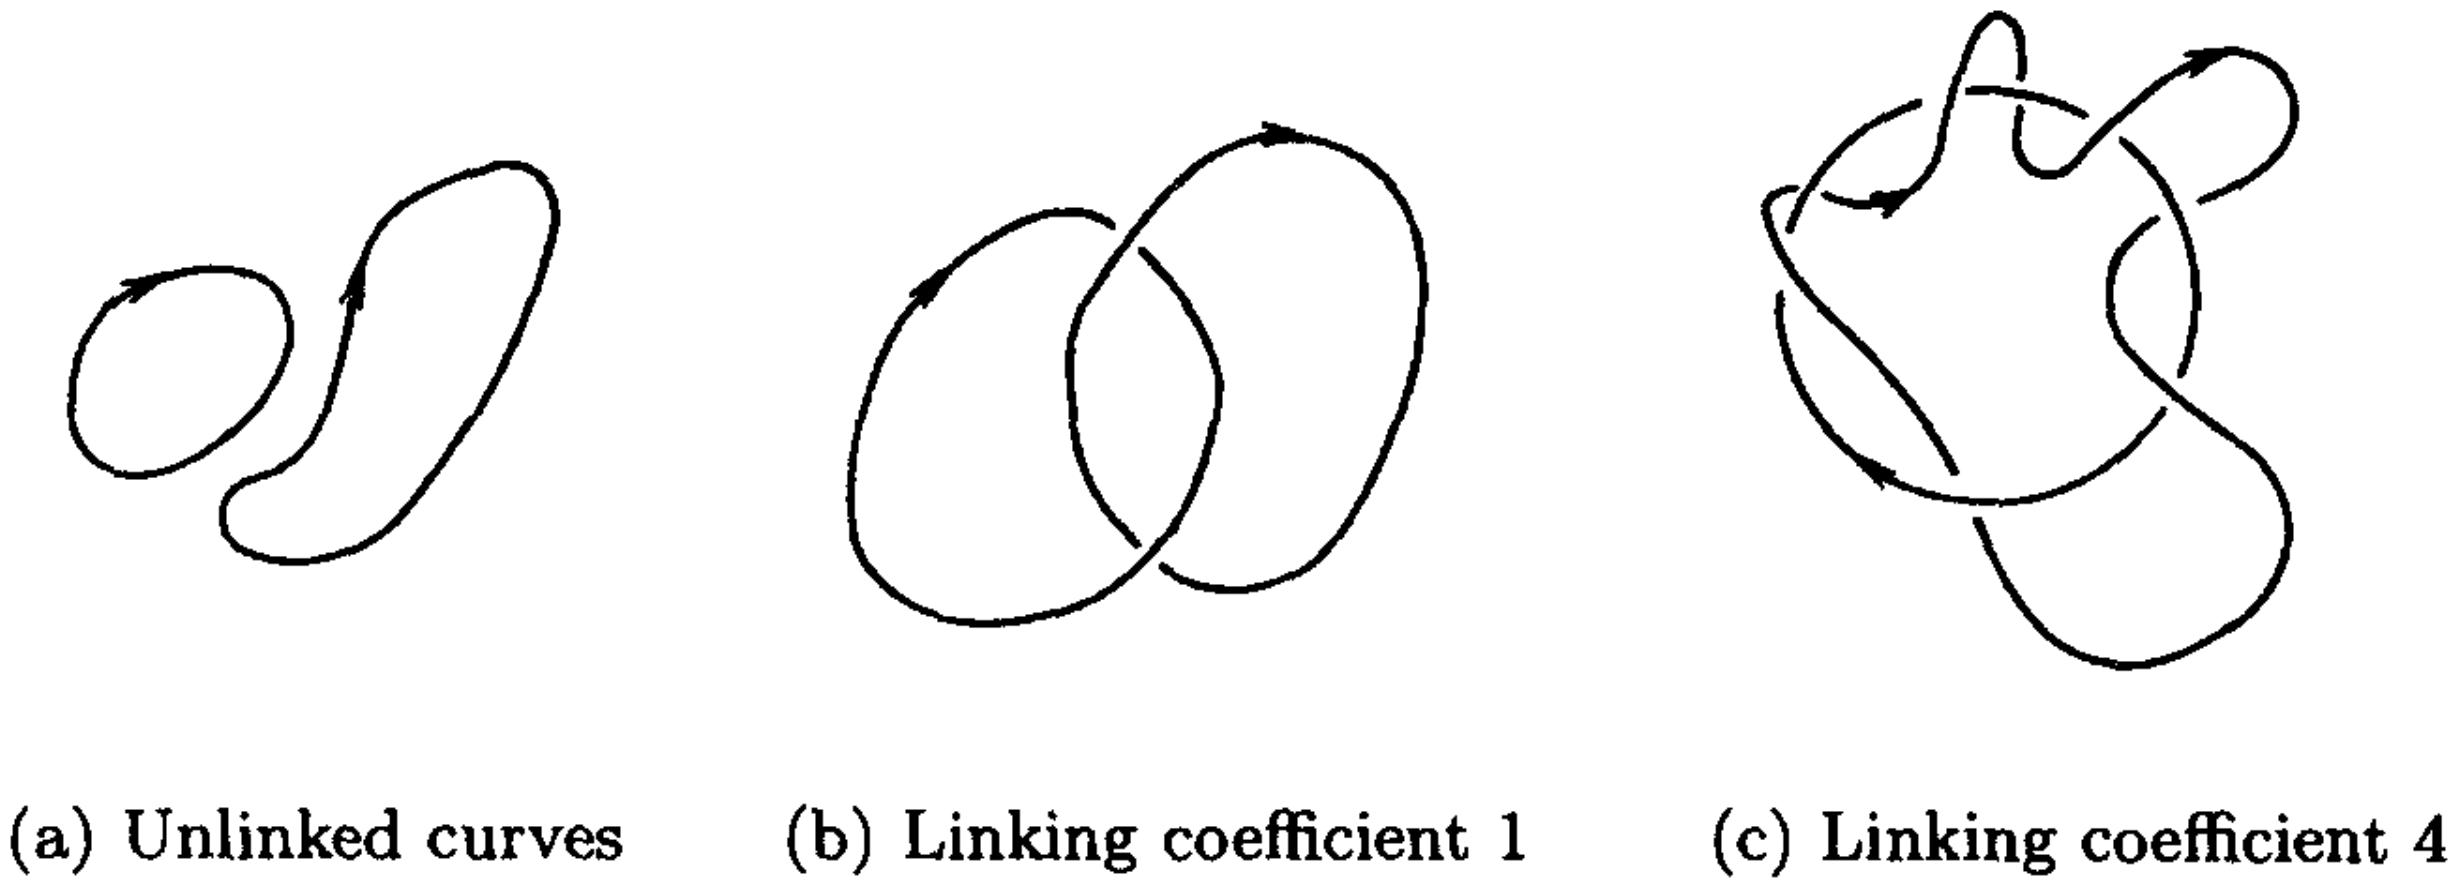
\includegraphics[width=0.86\textwidth]{figures/fig1_1.png}
\figtitle{1.1}{(a) 互不相环的两条曲线；(b) 环绕系数为 $1$；(c) 环绕系数为 $4$}
\end{figure}

% [原文 p.9]
Gauss 引入了由 $\R^3$ 中两条简单闭曲线 $\gamma_1,\gamma_2$ 构成的链环的一个不变量，即其中一条曲线绕另一条的带符号圈数，称为链环的\emph{环绕系数} $\{\gamma_1,\gamma_2\}$。他的公式是
\begin{equation}
N=\{\gamma_1,\gamma_2\}=\frac{1}{4\pi}\oint_{\gamma_1}\oint_{\gamma_2}
\frac{\bigl([d\gamma_1(t),d\gamma_2(t)],\gamma_1-\gamma_2\bigr)}
{\bigl|\gamma_1(t)-\gamma_2(t)\bigr|^3}, \tag{0.3}
\end{equation}
其中 $[\ ,\ ]$ 表示 $\R^3$ 中向量的向量（叉）积，$(\ ,\ )$ 表示欧氏数积。于是这个积分总是取整数值 $N$。若取其中一条曲线为 $\R^3$ 中的 $z$ 轴、另一条位于 $(x,y)$ 平面内，则公式 (0.3) 给出平面曲线绕 $z$ 轴的净圈数。

有趣的是，即使曲线非平凡地环绕，环绕系数 (0.3) 也可能为零（见图 1.2）。因此它的非零值只是环路非平凡环绕的一个充分条件。

% [Tutor Note: 注意 (0.3) 中分子是向量三重积 $([d\gamma_1,d\gamma_2],\gamma_1-\gamma_2)$，分母是两点距离的立方——量与量之间正好配成无量纲，被积表达式在重参数化下不变，所以 $N$ 是良定的整数。原书这里的 $\gamma_1,\gamma_2$ 在积分号内省略了参数 $t,\tau$，初读容易把 $\gamma_1-\gamma_2$ 误当常数向量。]

\begin{figure}[htbp]
\centering
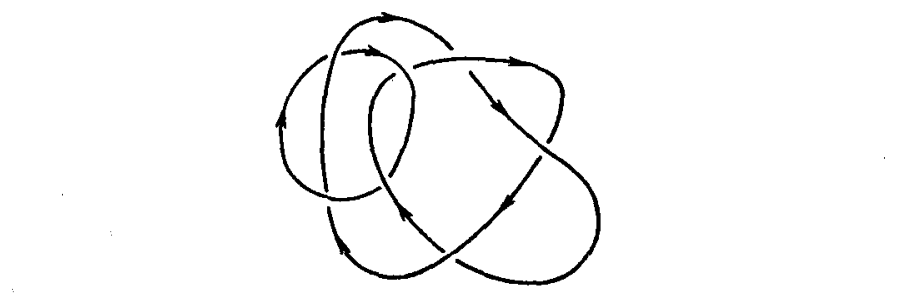
\includegraphics[width=0.52\textwidth]{figures/fig1_2.png}
\figtitle{1.2}{环绕系数等于 $0$，但两条曲线非平凡地环绕}
\end{figure}

% [原文 p.10]
早在 19 世纪这门学科创立之初，道路及其间同伦的初等拓扑性质就在复分析中起了重要作用。它们无疑是复变函数论最重要的特征之一，是该理论在一切应用中获得实效与成功的关键。复解析函数 $f(z)$ 常常只在复平面的一部分上才有定义并且单值，即在某个不含极点、分支点等的区域 $U\subset\R^2$ 上如此。沿每条闭围道 $\gamma\subset U$ 的 Cauchy 积分给出围道的一个「拓扑」泛函：
\begin{equation}
I_f(\gamma)=\oint_\gamma f(z)\,dz, \tag{0.4}
\end{equation}
意思是：在区域 $U$ 内对曲线 $\gamma$ 作连续同伦（形变）时，只要形变避开了函数的奇点，积分就保持不变。正是这种自由度——可以在不影响积分值的前提下形变闭围道——为各种应用开辟了巨大的空间。

更复杂的拓扑现象在 19 世纪出现了——本质上始于 Abel 与 Riemann——它们与复变量函数 $f(z)$ 的研究有关，而这函数只由一个方程隐式给出：
\begin{equation}
F(z,w)=0,\qquad w=f(z), \tag{0.5}
\end{equation}
或者由最初只在平面某部分上解析且单值的函数经整个平面上的解析延拓而给出。前一种情形以特别尖锐的形式出现（Riemann 与 Poincaré 之后这一点已经清楚），其背景是 Abel 对著名的「一般代数方程不可根式解」问题的解决；此时函数 $F(z,w)$ 是二元多项式：
\begin{equation}
F(z,w)=w^n+a_1(z)w^{n-1}+\cdots+a_n(z)=0. \tag{0.6}
\end{equation}
这样一个多项式方程一般在平面内有有限多个孤立的分支点 $z_1,\dots,z_m$，在这些点之外它恰有 $n$ 个不同的根 $w_j(z)$，$z\ne z_k$（$k=1,\dots,m$）。这里区域 $U$ 就是去掉这 $m$ 个分支点后的平面：
\[
U=\R^2\setminus\{z_1,\dots,z_m\}.
\]
结果表明，一般说来分支点不能被简单地忽略，理由如下。在不等于分支点的每一点 $z_0$ 的某个邻域内，方程 (0.6) 恰好确定 $n$ 个不同的函数 $w_j(z)$，使 $F(z,w_j(z))=0$。然而，若试图把其中任一 $w_j$ 解析延拓到这个邻域之外，就会遇到如下困难：沿一条绕过某些分支点又回到 $z_0$ 的道路延拓 $w_j$ 时，可能得到非平凡的单值性（monodromy），即在 $z_0$ 处到达另一个解：
\[
w_s(z_0)\ne w_j(z_0),\qquad s\ne j.
\]
% [原文 p.11]
更系统地考虑：取区域 $U=\R^2\setminus\{z_1,\dots,z_m\}$ 中所有可能的环路 $\gamma(t)$，$a\le t\le b$，且 $\gamma(a)=\gamma(b)=z_0$。每个这样的环路确定函数 $w(z)$ 的各分支的一个置换：如果从由 $w_j(z)$ 给出的分支出发、沿环路从 $a$ 走到 $b$，那么当 $t=b$ 时我们到达由 $w_s$ 定义的分支，于是环路 $\gamma(t)$ 确定了 $z_0$ 上方各分支（各\emph{叶}）的一个置换 $j\to s$：
\[
\gamma\to\sigma_\gamma,\qquad \sigma_\gamma(j)=s.
\]
反向道路 $\gamma^{-1}$（即从 $b$ 反向追溯到 $a$ 的道路）给出逆置换 $\sigma_\gamma^{-1}:s\to j$；两条道路 $\gamma_1$（从时刻 $a$ 走到时刻 $b$）与 $\gamma_2$（从 $b$ 走到 $c$）的叠置 $\gamma_1\cdot\gamma_2$，即先走 $\gamma_1$ 再接 $\gamma_2$ 得到的道路，对应于相应置换的乘积：
\begin{equation}
\sigma_{\gamma_1\cdot\gamma_2}=\sigma_{\gamma_2}\circ\sigma_{\gamma_1},\qquad
\sigma_{\gamma^{-1}}=(\sigma_\gamma)^{-1}. \tag{0.7}
\end{equation}
在一般的非退化情形，形如 $\sigma_\gamma$ 的置换生成 $n$ 个符号的完整对称群。（这就是代数方程 (0.6) 当 $n\ge 5$ 时一般不能根式求解的深层原因。）要看出这一点，注意「基本」道路 $\gamma_j$，$j=1,\dots,m$（它从 $z_0$ 出发、绕单个分支点 $z_j$ 一圈、再沿同一初始线段回到 $z_0$，见图 1.3），在分支点处于最大非退化状态这一典型情形，对应于两叶的互换（即 $\sigma_{\gamma_j}$ 只是两个指标的换位）。于是断言就由「换位生成全部置换」这一事实推出。

\begin{figure}[htbp]
\centering
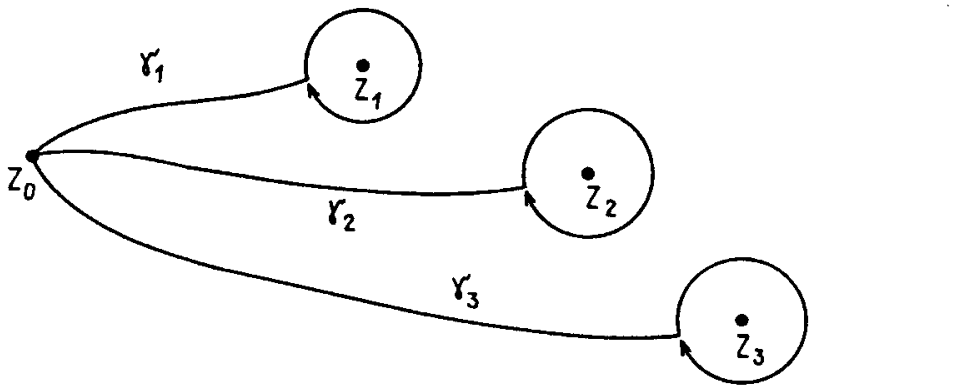
\includegraphics[width=0.72\textwidth]{figures/fig1_3.png}
\figtitle{1.3}{分支点 $z_1,z_2,z_3$ 与基本道路 $\gamma_1,\gamma_2,\gamma_3$}
\end{figure}

值得注意的是，若在 $U$ 内对环路 $\gamma$ 作连续同伦而始终保持起点与终点在 $z_0$，则置换 $\sigma_\gamma$ 不变。这与 Cauchy 积分在同伦下的不变性（见上文 (0.4)）类似，但在代数上更复杂：置换 $\sigma_\gamma$ 对道路 $\gamma$ 的依赖是非交换的，与 Cauchy 积分相反：
\begin{equation}
\sigma_{\gamma_1\cdot\gamma_2}=\sigma_{\gamma_2}\circ\sigma_{\gamma_1}\ne\sigma_{\gamma_2\cdot\gamma_1},
\qquad I_f(\gamma_1\cdot\gamma_2)=I_f(\gamma_1)+I_f(\gamma_2). \tag{0.8}
\end{equation}
% [Tutor Note: (0.8) 右端写的是 $\sigma_{\gamma_2\cdot\gamma_1}$，而 $\gamma_1,\gamma_2$ 按前文定义只在 $\gamma_1(1)=\gamma_2(0)$ 时才能复合，故这里应读作「把两条道路的次序颠倒过来复合」，原书以此来显示 $\sigma$ 对道路的依赖是反序的（非交换性的要害）。若把 $\sigma_{\gamma_2\cdot\gamma_1}$ 当作「$\gamma_2$ 接 $\gamma_1$」的置换，则 (0.8) 左右两端都是同一个 $\sigma_{\gamma_2}\circ\sigma_{\gamma_1}$，不等式便失去意义。]
% [原文 p.12]
这类考虑自然地引出一个群，其元素是始于并终于某个固定点 $z_0\in U$ 的连续环路 $\gamma(t)$ 的同伦类；这里 $U$ 可以是任何区域，甚至任何流形、复形或拓扑空间。这个群称为 $U$ 的\emph{基本群}（基点取 $z_0$），记作 $\pi_1(U,z_0)$。于是由 $F(z,w)=0$ 定义的 Riemann 面给出从基本群到其「叶」（即 $z=z_0$ 邻域内函数 $w(z)$ 的各分支）的置换群的一个同态——单值性作用（monodromy）：
\begin{equation}
\sigma:\pi_1(U,z_0)\to S_n, \tag{0.9}
\end{equation}
其中 $S_n$ 表示 $n$ 个符号上的对称群，$U$ 如前，是 $\R^2$ 的一个区域。

另一方面，对超越函数 $F$，方程 $F(z,w)=0$ 可能确定一个有无穷多叶（$n=\infty$）的多值函数 $w(z)$。最简单的例子是
\[
F(z,w)=\exp w-z=0,\qquad U=\R^2\setminus\{0\},\qquad w=\ln z.
\]
在这个例子里，各叶借助整数以自然的方式编号：取 $z_0=1$，则 $w_k=\ln z_0=2\pi ik$，其中 $k$ 取遍整数。满足 $|\gamma|=1$、$\gamma(0)=\gamma(2\pi)=1$、沿顺时针方向恰好绕点 $z=0$ 一圈的道路 $\gamma(t)$，给出单值性作用 $\gamma\to\sigma_\gamma$，$\sigma_\gamma(k)=k-1$。

% [Tutor Note: 原书此处写 $U=\R^2\setminus 0$，是「去掉原点」的简写，应读作 $\R^2\setminus\{0\}$；$\ln$ 的各个单值分支在此按 $2\pi i$ 的整数倍编号，所以顺时针绕原点一圈使编号 $k$ 减 $1$——符号方向取决于定向约定，抄写时不要顺手改成 $k+1$。又，本句原书印作 $w_k=\ln z_0=2\pi ik$，而 $\ln z_0=\ln 1=0$，故应读作 $w_k(1)=2\pi ik$。]

纽结理论是基本群 $\pi_1(U,z_0)$ 的非交换性真正起作用的一个有趣例子：所论对象是 $\R^3$ 中光滑（或分片光滑、或分片线性，随你）的简单闭曲线 $\gamma(t)\subset\R^3$，$\gamma(t+2\pi)=\gamma(t)$。更一般地是前面已引入的链环理论，链环是 $\R^3$ 中有限个简单、闭、互不相交的曲线 $\gamma_1,\dots,\gamma_k$ 的集合。当 $k>1$ 时，有以环绕系数 $\{\gamma_i,\gamma_j\}$（$i\ne j$，由公式 (0.3) 给出）为元素的矩阵，然而它并不能确定链环的全部拓扑不变量。当 $k=1$、即纽结的情形，根本没有这样的系数可用。设 $\gamma$ 是一个纽结，$U$ 是纽结在 $\R^3$ 中的补区域：
\begin{equation}
U=\R^3\setminus\gamma. \tag{0.10}
\end{equation}
结果表明，基本群 $\pi_1(U,z_0)$（$z_0$ 为 $U$ 的任一点）是交换群，当且仅当给定纽结 $\gamma$ 能通过纽结的光滑同伦（即所谓「同痕」）变成平凡纽结。所谓平凡纽结，即平凡嵌入的圆 $S^1\subset\R^2\subset\R^3$（其中 $S^1$ 可位于例如 $(x,y)$ 平面内；见第 4 章 §5）。

% [原文 p.13]
初等纽结理论（见图 1.5）表明，对每个纽结，交换化基本群
\[
H_1(U)=\pi_1/[\pi_1,\pi_1]
\]
都是无限循环群，其中 $[\pi_1,\pi_1]$ 表示 $\pi_1$ 的换位子群，$U$ 如前是 $\R^3$ 中的纽结补集。更一般地，对链环 $\{\gamma_1,\dots,\gamma_k\}$，群 $H_1(U)$ 是 $k$ 个无限循环群的直和。对\emph{任何}拓扑空间 $U$，交换化基本群 $\pi_1/[\pi_1,\pi_1]$ 称为\emph{一维整同调群}，如上记作 $H_1(U)$，或记作 $H_1(U;\Z)$。$H_1$ 中的群运算总写成加法。

\begin{figure}[htbp]
\centering
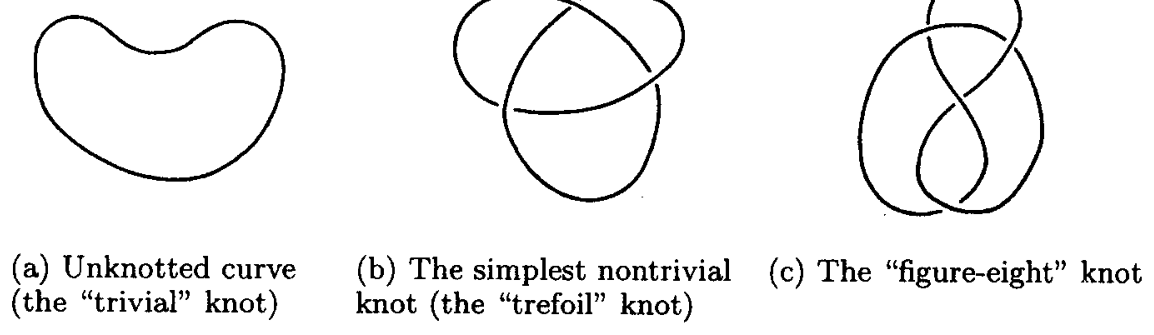
\includegraphics[width=0.8\textwidth]{figures/fig1_4.png}
\figtitle{1.4}{(a) 不打结的曲线（「平凡」纽结）；(b) 最简单的非平凡纽结（「三叶」纽结）；(c) 「八字」纽结}
\end{figure}

前面我们看到，在平面区域 $U\subset\R^2$ 中，$U$ 内单值解析函数（无极点！）沿 $U$ 中闭围道 $\gamma$ 的 Cauchy 积分
\[
I_f(\gamma)=\oint_\gamma f(z)\,dz
\]
确定了一维同调群 $H_1(U;\Z)$ 上的一个复值线性形式（特别见 (0.8)）。

用更现代的例子来结束我们这组初等拓扑观察是恰当的，这个例子来自 30 年代，即圆或弧上的奇异积分方程理论；它最初是二维弹性力学中几个重要的边值问题之一（Noether、Muskhelishvili）。后来，由于它在椭圆线性微分算子与伪微分算子理论的发展中起了相当大的作用，这一理论获得了重要得多的意义。设 $H_1,H_2$ 是 Hilbert 空间，$A:H_1\to H_2$ 是\emph{诺特算子}（现称 Fredholm 算子），即一个闭（且有界）线性算子，其核 $\Ker A=\{h\mid A(h)=0\}$ 有限维（不要与积分算子的核混淆！），且「余核」也有限维，即伴随算子 $A^*:H_2\to H_1$ 的核有限维。

% [原文 p.14]
结果表明，这种算子 $A$ 的\emph{指标} $i(A)$ 由
\begin{equation}
i(A)=\dim(\Ker A)-\dim(\Ker A^*) \tag{0.11}
\end{equation}
定义，即方程 $A(h)=0$ 与 $A^*(h^*)=0$ 各自线性无关解个数之差，是同伦不变量。这无非是说：指标 $i(A)$ 在算子 $A$ 的连续形变下保持不变，尽管 (0.11) 右端的各个维数可能会改变。

在积分算子 $\widehat K$ 的核 $K(x,y)$ 非奇异这一最简单情形，「Fredholm 二择一」是在本世纪初发现的。用泛函分析的语言，这实际上只是断言：对形如 $A=\widehat I+\widehat K$ 的算子，$i(A)=0$，其中 $\widehat K$ 是「紧算子」，即对 $H_1$ 的每个有界子集 $M$，$\widehat K(M)$ 是 $H_2$ 的紧子集，而算子 $\widehat I$ 是 Hilbert 空间 $H_1$ 与 $H_2$ 的同构。事实上，给任何诺特算子 $A$ 加上紧算子仍保持诺特性，因此诺特算子类中最简单的形变具有形式 $A_t=A_0+t\widehat K$（在经典 Fredholm 情形 $A_0=\widehat I$）。

另一方面，对奇异积分算子，指标是相当复杂的拓扑特征。20 年代与 30 年代的大量经典工作致力于通过算子的核显式计算指标。这一理论向高维流形的深远推广，最终凝聚为 Atiyah--Singer 指标定理，对拓扑学及其应用具有非同寻常的意义。

\begin{figure}[htbp]
\centering
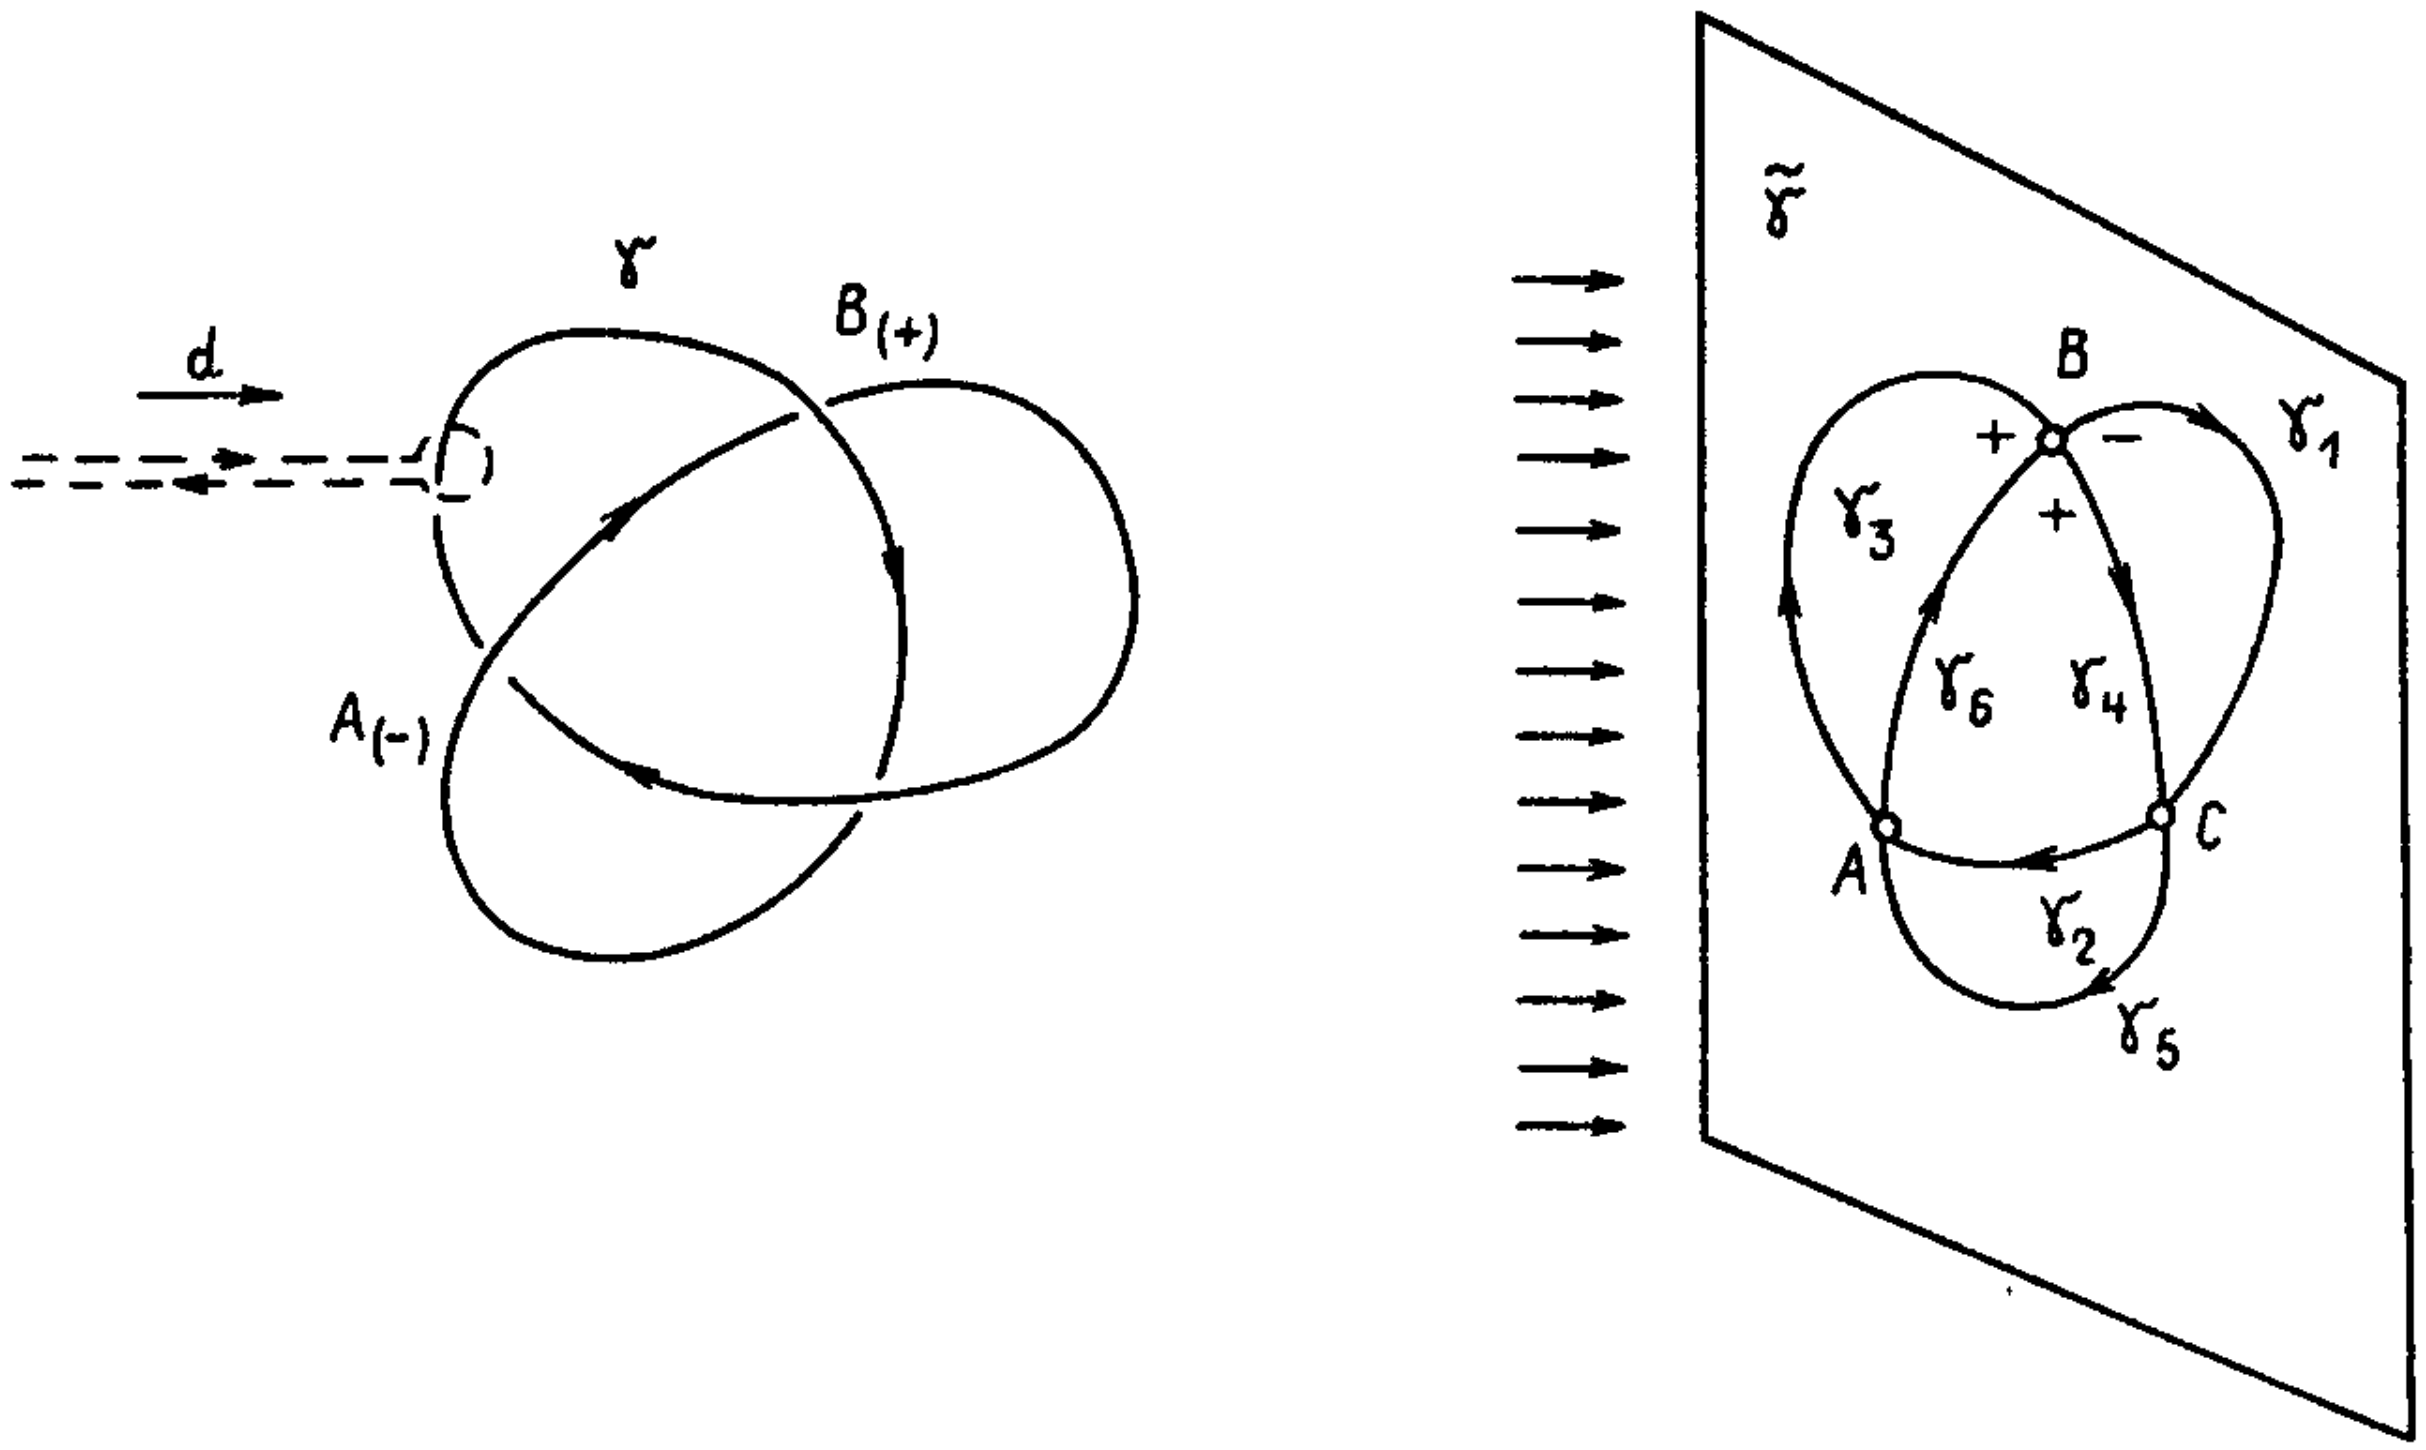
\includegraphics[width=0.78\textwidth]{figures/fig1_5.png}
\figtitle{1.5}{纽结的环绕与它在平面投影中的环路 $\gamma_1,\dots,\gamma_6$}
\end{figure}

% [原文 p.15]
这个例子说明，拓扑性质不仅在与直观意义上的几何图形有关时出现，也会在性质完全不同的数学背景中出现。

% CHUNK ch01 DONE
